\input ../talk-header.tex
\title
{Machine Learning}
\subtitle{Features and Modeling}

% If you wish to uncover everything in a step-wise fashion, uncomment
% the following command: 
%\beamerdefaultoverlayspecification{<+->}

\begin{document}

\begin{frame}
  \titlepage
\end{frame}

\begin{frame}
  \phrase{Vector spaces}

  \vspace{1cm}
  \only<2>{\centerline{Features are dimensions}}
\end{frame}

\begin{frame}
  \phrase{Feature extraction}

  \vspace{1cm}
  \phrase{Feature engineering}

  \only<2>{\vspace{3mm}\centerline{Synthetic features}}
\end{frame}

\begin{frame}
  \frametitle{Feature Engineering}
  \only<1>{
    \begin{enumerate}
    \item Brainstorm
    \item Pick some
    \item Make them
    \item Evaluate
    \item Repeat
    \end{enumerate}
  }
\end{frame}

\begin{frame}
  \vspace{4mm}
  
  \cimgh{titanic-titles.png}
  \vspace{-3mm}
  \prevwork{Kaggle}
\end{frame}

\begin{frame}
  \cimg{reading-time-1.png}
  \prevwork{Jellybooks}
\end{frame}

\begin{frame}
  \cimg{reading-time-2.png}
  \prevwork{Jellybooks}
\end{frame}

\begin{frame}
  \vphrase{One of $K$ = one-hot encoding}
\end{frame}

\begin{frame}
  \frametitle{Text features}
  \blue{Bag of words}
  \only<1>{
    \begin{itemize}
    \item Corpus (documents)
    \item Vocabulary (set of unique words)
    \item Words
    \end{itemize}
  }
  \only<2>{
    \begin{itemize}
    \item Order doesn't matter
    \item Stop words
    \item Stemming {\it(racinisation, désuffixation)}
    \item Lemmatisation {\it(transformer en lemme)}
    \end{itemize}
  }
\end{frame}

\begin{frame}
  \frametitle{Image features}
  \only<1>{
    \begin{itemize}
    \item Corners, edges (rotation invariant, but scaling can hide)
    \item More complex: scale space or RNN
    \item Point matching is easy
    \end{itemize}
  }
  \only<2>{
    Problems
    \begin{itemize}
    \item Illumination
    \item Scale
    \item Rotation
    \item Skew (perspective)
    \item Data size (matrices not sparse)
    \end{itemize}
  }
\end{frame}

\begin{frame}
  \frametitle{python}
  \only<1>{Useful tools
    \begin{itemize}
    \item virtualenv
    \item pip
    \item ipython
    \item ipython notebook
    \item \url{conda.pydata.org}
    \end{itemize}
  }
  \only<2>{Notes
    \begin{itemize}
    \item \texttt{pip install -r requirements.txt}
    \item ipython offers tab completion (vs python)
    \item ipython notebook opens in a browser, caches cell output but not cell state
    \end{itemize}
  }
\end{frame}

\begin{frame}
  \frametitle{pandas}
  \only<1>{\lstinputlisting{pandas_1.py}}
  \only<2>{\purple{\texttt{Dataframe} has many constructors.  For example,}
    \lstinputlisting{pandas_2.py}
  }
  \only<3>{\purple{Viewing data}
    \lstinputlisting{pandas_3.py}
  }
  \only<4>{\purple{Basic data exploration}
    \lstinputlisting{pandas_4.py}
  }
  \only<5>{\purple{Select a column (series)}
    \lstinputlisting{pandas_5.py}
  }
  \only<6>{\purple{Select a range}
    \lstinputlisting{pandas_6.py}
  }
  \only<7>{\purple{Boolean selection criteria}
    \lstinputlisting{pandas_7.py}
  }
  \only<8>{\purple{Recommended}
    
    \vspace{5mm}
    \url{http://www.gregreda.com/2013/10/26/intro-to-pandas-data-structures/}
  }
\end{frame}

\begin{frame}
  \frametitle{Plotting}
  \only<1>{\purple{Draw a line}
    \lstinputlisting{pyplot_1.py}
    \vspace{-19mm}
    \flushright{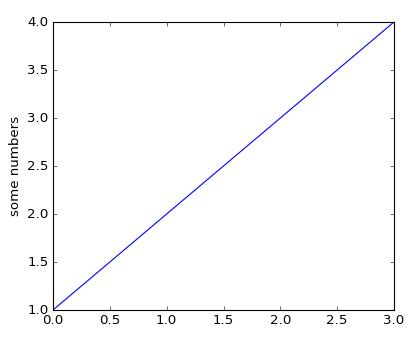
\includegraphics[width=.5\textwidth]{pyplot_1.png}}
  }
  \only<2>{\purple{Draw a line}
    \lstinputlisting{pyplot_2.py}
    \vspace{-19mm}
    \flushright{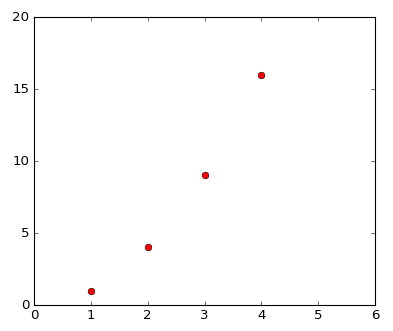
\includegraphics[width=.5\textwidth]{pyplot_2.png}}
  }
  \only<3>{\purple{Draw a line}
    \lstinputlisting{pyplot_3.py}
    \vspace{-55mm}
    \flushright{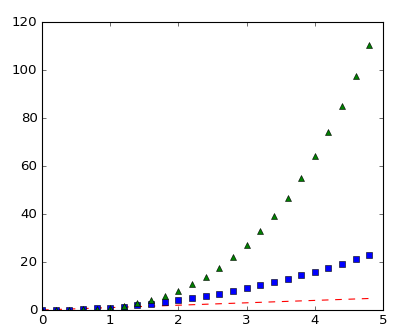
\includegraphics[width=.5\textwidth]{pyplot_3.png}}
  }
  \only<4>{\purple{Draw two curves}
    \lstinputlisting{pyplot_4.py}
  }
  \only<5>{
    \flushright{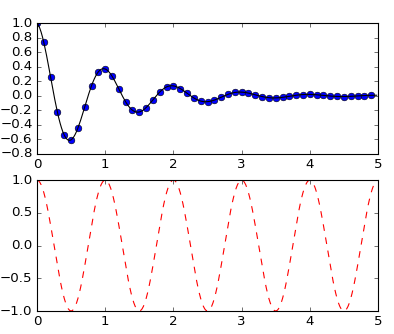
\includegraphics[width=.5\textwidth]{pyplot_4.png}}
  }    
  \only<6>{\purple{Draw two curves}
    \lstinputlisting{pyplot_5.py}
  }
  \only<7>{
    \flushright{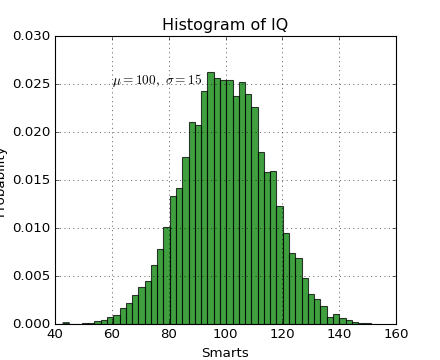
\includegraphics[width=.5\textwidth]{pyplot_5.png}}
  }
  \only<8>{\purple{Scatter plot}
    \prevwork{\url{http://matplotlib.org/mpl_examples/pylab_examples/scatter_demo2.py}}
    \lstinputlisting{pyplot_6.py}
    \vspace{-60mm}
    \flushright{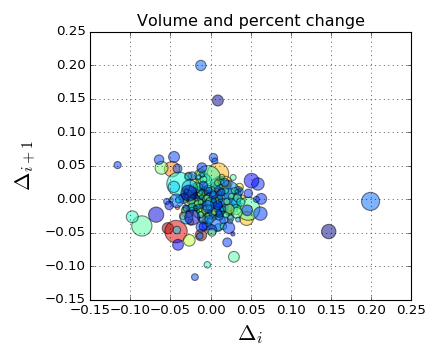
\includegraphics[width=.5\textwidth]{pyplot_6.png}}
    
  }
  \only<9>{
    \prevwork{\url{http://matplotlib.org/users/pyplot_tutorial.html}}
      
    \prevwork{\url{http://matplotlib.org/users/beginner.html}}
  }
\end{frame}

%%%%%%%%%%%%%%%%%%%%%%%%%%%%%%%%%%%%%%%%%%%%%%%%%%%%%%%%%%%%%%%%%%%%%%
%\talksection{Break}

\begin{frame}
  % https://www.pexels.com/photo/food-healthy-people-woman-41219/
  % https://static.pexels.com/photos/41219/apple-diet-face-food-41219.jpeg
  % CC0 license
  \cimgh{apple-pear.jpg}
  \vspace{-.6\textheight}
  \phrase{Questions?}
\end{frame}

\end{document}
